\subsection{违约定义}
\begin{frame}{展期不算违约?}
	近几个月来,房地产企业暴雷不断,有人因此提出“展期不算违约”,阳光城、奥园等地产企业及恒大上游供应商南通三建等纷纷进行展期的操作。

	但展期延长还款本质上仍然违反了债券签订时的合同,侵害投资者利益,并且展期最后是否能真正还款仍有很大变数。因此我们认为展期也算作违约。类似的,所谓“技术性违约”,我们也认为属于违约。

	此外,花式躲避违约的方式还有“场外兑付”。历史上看,选择过“场外兑付”的中融新大、山东如意最终都无可挽回的走向了公开市场债券违约。“场外兑付”能否保证投资者利益、避免交叉违约作用存疑。并且不通过交易所直接将利息付给投资者数额不会披露,不一定足额付息,显然违反了债券合同成立时的规则。因此我认为“场外兑付”也算违约。
	\begin{quote}
		恒大地产日公告称,已通过场外方式协商解决关于9月23日到期的“20恒大04”债劵到期利息,该债劵利息共计约2.32亿元。
	\end{quote}
\end{frame}
\begin{frame}{评级}
	\small{\small {尽管\citet{梅冬州2021财政扩张} 论证了机构机构投资者将评级机构的债券评级作 为投资门槛条件,而在做具体决策时则主要通过自己的内部评级和定价分析体系,是因为评级机构评级失真。

			评级机构事前很难公正评级,很多情况下事后才下调评级。但反过来说,下调评级通常包含着信用问题已经比较严重了的信息。因此我们会关注评级是否下调,而不关注评级具体数值和上升的情况。}}
	\begin{figure}
		\centering
		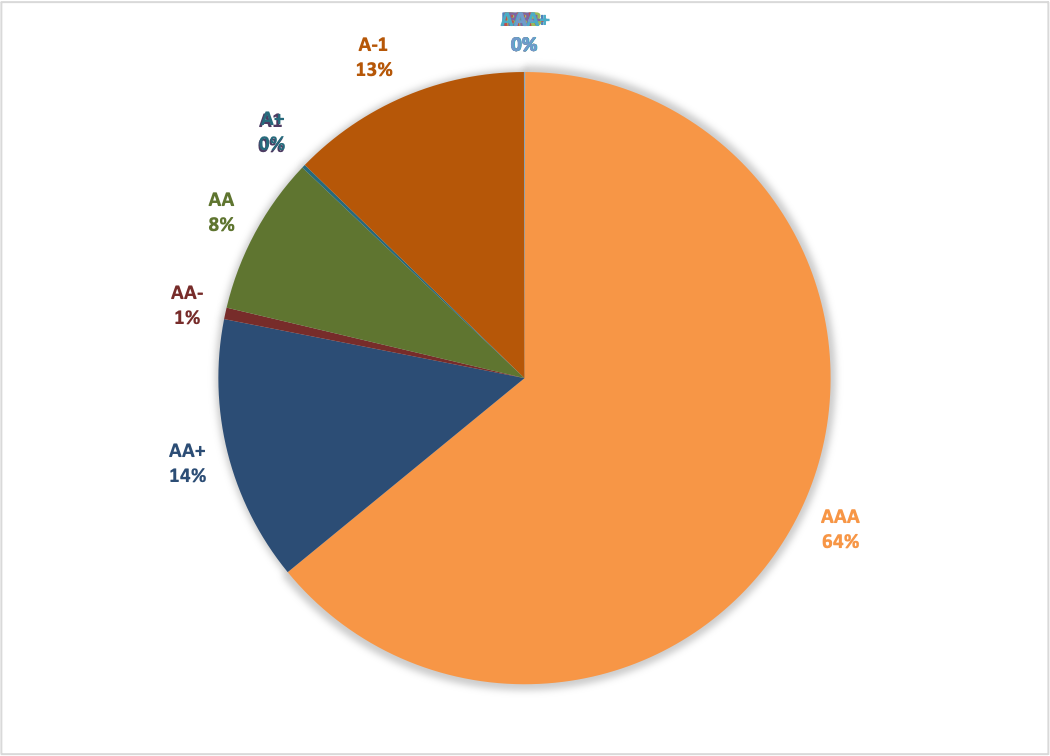
\includegraphics[width=0.6\linewidth]{lib/rating.png}
		\caption{2014年以来评级分布(按金额计)}
	\end{figure}
\end{frame}
\subsection{数据来源及分析}
\begin{frame}
	主要数据来自于 wind 数据库。

	描述性统计 TBA
\end{frame}
\subsection{Logit回归检验}
\label{Logit}
\begin{frame}{回归}
	控制变量:
	\begin{itemize}
		\item 久期
		\item ?
	\end{itemize}
	回归:
	\begin{equation*}
		DEFAULT = \alpha + \beta_1 X_{macro} + \beta_2 X_{industry} + \beta_3 X_{enterprise} + \beta_4 X_{bond} + \beta_5 Control
	\end{equation*}

\end{frame}
\subsection{机器学习加入非线形因素}
\begin{frame}{随机森林算法}
	首先采用决策树降维,梳理哪些因素可能导致违约,并和节\ref{Logit}对比。

	随机森林需要的样本量相对较小,结果比较稳健。

	但采用随机森林方法,结果无法解释。训练结果与节\ref{Logit}比对。
\end{frame}
